\section{Problem}

A typical crossword involves a grid with black squares, not to be filled in by the
 solver, and white squares used by the solver to input their answers. The input
 comes from the solver working out the answer to given clues, these clues have
 an orientation, a length and a number associated with its related position within
 the grid. The fundamental difference between a typical crossword and a cryptic
 crossword are the clues themselves. 

Cryptic crosswords are a popular type of puzzles found in many parts of the
 world. Most common-wealth national newspapers will print cryptic crosswords 
of varying difficulty on a daily basis.

Cryptic crosswords are a unique style of crosswords, in which the answer to 
each given clue is a word puzzle. An answer can only be obtained if the cryptic
 clue is read in the correct way. Often when the clue is surface read, the clue
 makes no sense at all. The challenge is to find a way in which the reading of 
the clue leads to a solution. To aid with solving cryptic crosswords, the clues
 are written to be within specific categories, such as reversals and anagrams,
 which have individual characteristics. 

Many users can often become frustrated when a clue appears to be unsolvable. It
is the vast range of possible clues that often makes solving not only 
challenging but interesting as well.

Fundamentally, the overall aim of this project is to develop a piece of 
software that is able to solve any given type of cryptic crossword clue.


\section{Product}
Within this group project, two components will be delivered. The first is a 
written report comprising of the all research and implementation details of 
the software product. The second deliverable is the final, working piece of software.

Based upon the given background and problem information it could be possible
 to develop a product that is able to solve the given problem.

The final product would be a piece of software that is able to understand 
a given clue and try to deduce what the answer to the clue is. This would require
 the software to have some form of natural language processing component 
as well as one or more cryptic crossword algorithms. Once a clue has been
 correctly ``guessed'' it can simply be returned to the 
user. It is the ``guessing'' of the answer that this project will primarily 
focus upon.

In order to gain maximum user coverage, the software must have an easy to use interface.
 The main reason for this is that the computer literacy of the intended users is not
 known - although basic computer literacy is assumed.

\section{Client \& Stakeholders}
Dr Hugh Osborne, a lecturer from the University of Huddersfield will be 
the client for the group project. Dr Hugh Osborne has a keen interest in
 cryptic crosswords and the problem in the area which the group intends
 to help to eliminate. The role of the client for the group project will be to
 input ideas and potential requirements which Dr Hugh Osborne, as an
 experienced solver of cryptic crosswords, would consider to be necessary.
 As a client for the project, Dr Hugh Osborne will also be present for academic
 demonstrations.

Dr Gary Allen, Sotirios Batsakis and Colin Venters, all lecturers at the
 University of Huddersfield, will act as stakeholders for the group project.
 Dr Gary Allen will be the most involved external individual as the project 
supervisor. The role of project supervisor requires frequent meetings with the
 team to monitor the development of the project, provide guidance as well as 
opinion on certain aspects of the life cycle.  

Sotirios Batsakis and Colin Venters, will have a less active role within the project
 during the project life cycle than the role of the client or the project supervisor. 
These stakeholders will play active roles at particular milestones of the group 
project such as providing guidance for the proposal of the project and at the
 project demonstration approximately half way through the life cycle. 


\section{Users} 
Kathryn Friedlander and Philip Fine \citep{friedlander09} carried out an investigation into
whether the amount of cryptic crosswords completed by a solver determined how successful they
were at solving them.
To complete this study they gathered data from 241 people, this data can be used as part of
research to determine the typical audience cryptic crosswords have.
10
The following facts about the user base are taken from the results section of the paper \citep{friedlander09}:
\begin{itemize}
    \item ``209 M, 32 F''
    \item ``mean age=53 years, range=23-83''
    \item ``mean time spent=8 hours per week, range=1-30''
\end{itemize}

To support decisions made within the project life cycle an additional qualitative 
research method has  been utilized to gain a larger understanding of the
 types of users the deliverable will attract. The research method used by the
 team is in the form of a survey. The survey results gathered were seen as 
potentially additional justifications for the purpose of the project. Moreover, 
data collected from the survey was expected to indicate the locations in which
 users complete cryptic crosswords to understand the potential need for the deliverable
 to be of a transportable nature. 

The following questions were asked:
\begin{enumerate}
\item Do you play Cryptic Crosswords?
\item How often do you play?
\item Where do you play?
\item Do you often finish them?
\item If no to the previous question, what reason don't you finish them?
\item What is your age group?
\item When do you play Cryptic Crosswords?
\item What gender are you?
\item What is the Highest qualification you have?
\item What platform is your mobile phone on?
\end{enumerate}

The survey was conducted between (date) and (date). It was distributed across the Department
of Computing And Engineering at the University Of Huddersfield, Facebook and Twitter. The
results of this survey are shown in Figure 1.1.

\subsection{Results}
\begin{figure}[H]
\begin{center}
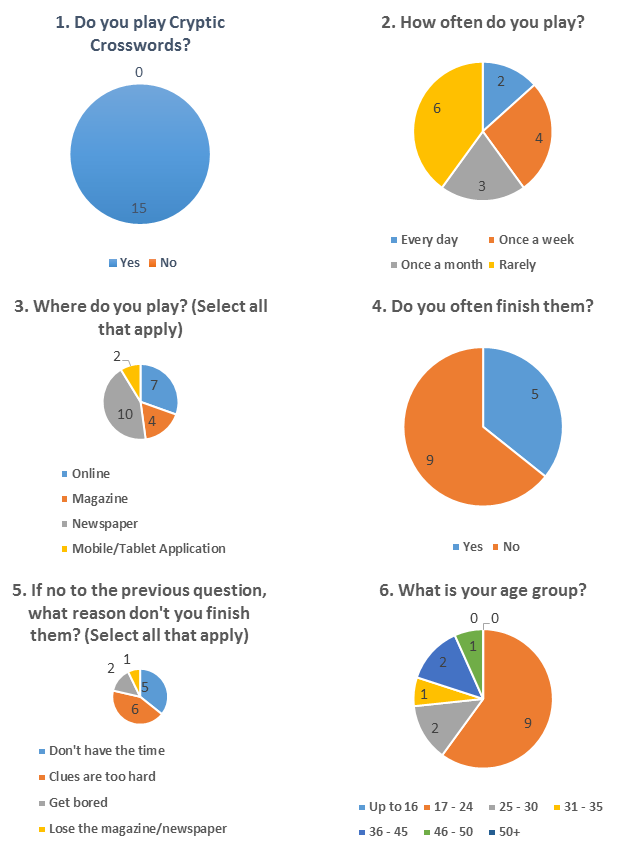
\includegraphics[keepaspectratio=true]
	{problem_analysis/graphs_1_6.png}
\caption{Results for survey questions 1 - 6}
\end{center}
\end{figure}

\begin{figure}[H]
\begin{center}
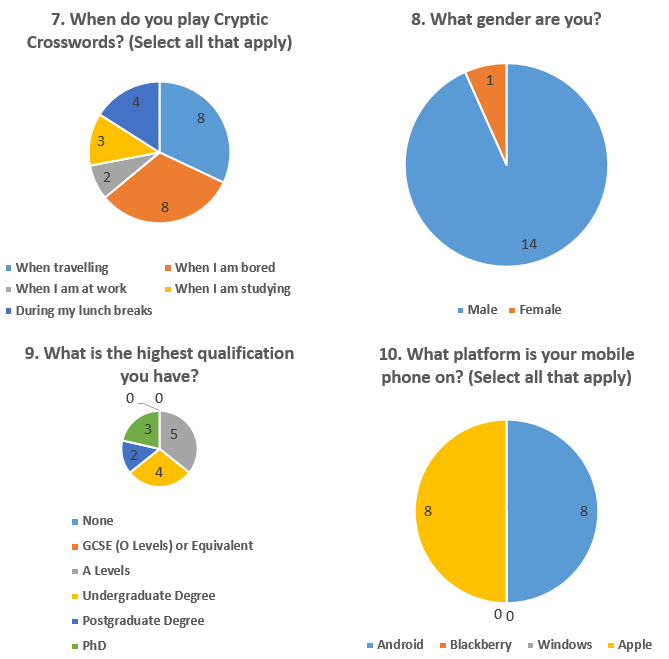
\includegraphics[keepaspectratio=true]
	{problem_analysis/graphs_7_10.png}
\caption{Results for survey questions 7 - 10}
\end{center}
\end{figure}



From these results it can be deduced that .....

